% Created 2023-08-30 Wed 14:32
% Intended LaTeX compiler: pdflatex
\documentclass[11pt,oneside]{memoir}
\makeatletter

\usepackage{answerkey-env}

\ifanswerkey
  \usepackage[forcolorpaper, answerkey]{eqexam}
  \usepackage{vinaya-class-questions}
\else
  \usepackage[forcolorpaper, nosolutions]{eqexam}
  \usepackage[nosolutions]{vinaya-class-questions}
\fi

\proofingsymbolColor{linkred}
\fillinColor{linkred}

\def\maketitle{}

\maxtocdepth{subsection}

\newenvironment{twocols}{%
  \raggedright%
  \setlength{\parindent}{0pt}%
  \setlength{\parskip}{8pt}%
  \fontsize{11}{17}\selectfont%
  \begin{multicols}{2}%
}{%
  \end{multicols}%
}

\newenvironment{widecols}{%
  \hspace*{-0.05\linewidth}\begin{minipage}{1.1\linewidth}%
  \raggedright%
  \setlength{\parindent}{0pt}%
  \setlength{\parskip}{8pt}%
  \fontsize{11}{17}\selectfont%
  \begin{multicols}{2}%
}{%
  \end{multicols}%
  \end{minipage}%
}

\newlength\@tmp@width
\newlength\@tmp@height

\renewcommand*{\printchaptertitleHook}{%
  \AddToShipoutPictureBG*{%
    \put(\LenToUnit{\paperwidth-25mm-\spinemargin},\LenToUnit{\paperheight-95mm}){%
      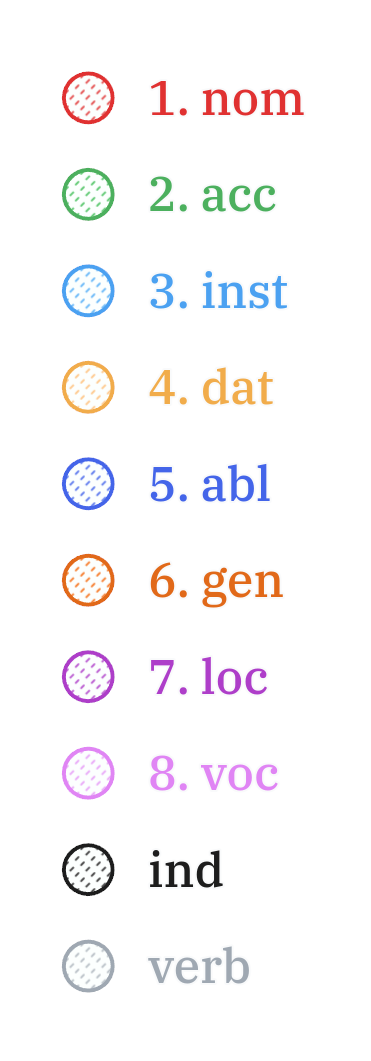
\includegraphics[width=25mm]{./images/cases-legend-white-large.png}%
    }%
  }%
}

\newcommand*\sentenceDiaMsg{\textbf{Exercise:} Draw a sentence analysis diagram below and indicate declensions.}

\newcommand*\sentenceDiaSolution[2][0.4]{%
  \ifanswerkey%
    \hspace*{-\spinemargin}%
    \begin{minipage}{\paperwidth}%
      \centering%
      \includegraphics[scale=#1]{#2}%
    \end{minipage}%
  \else%
    \settototalheight{\@tmp@height}{\includegraphics[scale=#1]{#2}}%
    \begin{minipage}[\@tmp@height]{\linewidth}%
      \sentenceDiaMsg%
    \end{minipage}%
  \fi%
}

\usepackage{cwpuzzle}

\renewcommand\PuzzleCluePre{%
  \begin{minipage}[t]{0.75\linewidth}%
}

\renewcommand\PuzzleClueFont{\fontsize{11}{17}\selectfont}

% \def\PuzzleThickline{\linethickness{2pt}}

\makeatother

\date{\today}
\title{Pali Readings}
\hypersetup{
 pdfauthor={The Bhikkhu Saṅgha},
 pdftitle={Pali Readings},
 pdfkeywords={},
 pdfsubject={},
 pdfcreator={Emacs 30.0.50 (Org mode 9.6.6)}, 
 pdflang={En_Gb}}
\begin{document}

\maketitle
\frontmatter

{\centering

{\Huge Pāḷi Readings}

\bigskip
\href{https://vinaya-class.github.io}{https://vinaya-class.github.io}

{\scshape\small last updated on}\\
\today

}

\bigskip
\tableofcontents*

\mainmatter

\yournamefalse

\newlength{\colOne}\setlength{\colOne}{0.35\linewidth}
\newlength{\colTwo}\setlength{\colTwo}{0.6\linewidth}

\chapter{Ratana Sutta Paritta (Snp 2.1)}
\label{sec:org4427bac}

\begin{spacedquote}
Yaṁ kiñci vittaṁ idha vā huraṁ vā, \\[0pt]
Saggesu vā yaṁ ratanaṁ paṇītaṁ; \\[0pt]
Na no samaṁ atthi tathāgatena, \\[0pt]
Idampi buddhe ratanaṁ paṇītaṁ; \\[0pt]
Etena saccena suvatthi hotu.
\end{spacedquote}

\begin{longtable}{L{\colOne} L{\colTwo}}
yaṁ \ldots{} taṁ \ldots{} & what \ldots{} that \ldots{}\\[0pt]
yaṁ kiñci (ind.) [yaṁ + kiṁ + ci] & whatever; everything; all\\[0pt]
vitta (nt.) & (1) wealth; property (2) delight; pleasure; lit. got\\[0pt]
huraṁ (ind.) & there; in another world\\[0pt]
sagga (m.) & heaven; paradise\\[0pt]
ratana (nt.) & (1) jewel; gem (2) treasure (3) queen\\[0pt]
paṇīta (adj.) & fine; superior; sublime; lit. brought forward\\[0pt]
sama (adj.) & (1) level; even; balanced (2) like; equal (to); same (as)\\[0pt]
sacca (nt.) & truth\\[0pt]
suvatthi (f.) [su + √as + ti] & well being; prosperity\\[0pt]
\end{longtable}

\begin{spacedquote}
Khayaṁ virāgaṁ amataṁ paṇītaṁ, \\[0pt]
Yadajjhagā sakyamunī samāhito; \\[0pt]
Na tena dhammena samatthi kiñci, \\[0pt]
Idampi dhamme ratanaṁ paṇītaṁ; \\[0pt]
Etena saccena suvatthi hotu.
\end{spacedquote}

\enlargethispage{\baselineskip}

\begin{longtable}{L{\colOne} L{\colTwo}}
khīyati & is destroyed; is exhausted\\[0pt]
khīṇa (pp. of khīyati) & consumed; destroyed\\[0pt]
khaya (m. from khīyati) & wearing away; destruction\\[0pt]
virāga (m.) & fading of desire (for); dispassion (towards)\\[0pt]
amata (nt.) & (1) deathless state; immortality (2) deathless; immortal; undying\\[0pt]
adhigacchati & gets to; attains; obtains; lit. arrives at\\[0pt]
ajjhagā (imperf. of adhigacchati) & got; obtained; achieved; lit. arrived at\\[0pt]
samādahati & (1) (of the mind) composes; stabilizes; collects (2) (of fire) kindles; lights; lit. puts together\\[0pt]
samāhita (pp. of samādahati) & composed; centred; settled\\[0pt]
\end{longtable}

\clearpage

\begin{spacedquote}
Yaṁ buddhaseṭṭho parivaṇṇayī suciṁ, \\[0pt]
Samādhimānantarikaññamāhu; \\[0pt]
[samādhiṁ + ānantarikaṁ + yaṁ + āhu] \\[0pt]
Samādhinā tena samo na vijjati, \\[0pt]
Idampi dhamme ratanaṁ paṇītaṁ; \\[0pt]
Etena saccena suvatthi hotu.
\end{spacedquote}

\begin{longtable}{L{\colOne} L{\colTwo}}
seṭṭha (adj.) & (1) foremost; supreme; (2) chief; leader\\[0pt]
vaṇṇayati & (1) praises; extols (2) comments on; interprets; explains\\[0pt]
parivaṇṇayati & describes; recommends; extolls; lit. praises all around\\[0pt]
suci (adj.) & (1) clean; pure (2) (of tastes and smells) good; fine\\[0pt]
antara (nt.) & space between; interval; distance\\[0pt]
ānantarika (adj.) & immediate; without delay; with immediate results\\[0pt]
√ah & (√) speak\\[0pt]
āhu (perf.3rd.pl. of āha) & they say; lit. they said\\[0pt]
vijjati [√vid + ya + ti] & (1) exists; is found; is present (2) is possible\\[0pt]
\end{longtable}

\begin{spacedquote}
Ye puggalā aṭṭha sataṁ pasatthā, \\[0pt]
Cattāri etāni yugāni honti; \\[0pt]
Te dakkhiṇeyyā sugatassa sāvakā, \\[0pt]
Etesu dinnāni mahapphalāni; \\[0pt]
Idampi saṅghe ratanaṁ paṇītaṁ, \\[0pt]
Etena saccena suvatthi hotu.
\end{spacedquote}

\begin{longtable}{L{\colOne} L{\colTwo}}
ye \ldots{} te \ldots{} & who \ldots{} they \ldots{}\\[0pt]
puggala (m.) & person; individual\\[0pt]
santa (m. irreg, from atthi) & virtuous man; good person (from √as)\\[0pt]
sataṁ (m.dat.pl. of santa, irreg) & for virtuous people; for good people\\[0pt]
pasaṁsati & praises; approves (of); commends\\[0pt]
pasattha (pp. of pasaṁsati) & praised; commended; exalted\\[0pt]
yuga (nt.) & (1) yoke (2) pair; set of two\\[0pt]
dadāti & gives (to); offers (to)\\[0pt]
dinna (pp. of dadāti) & given (to); offered (to)\\[0pt]
phala (nt.) & (1) fruit; berry (2) consequence; result\\[0pt]
\end{longtable}

\clearpage

\begin{spacedquote}
Ye suppayuttā manasā daḷhena, \\[0pt]
Nikkāmino gotamasāsanamhi; \\[0pt]
Te pattipattā amataṁ vigayha, \\[0pt]
Laddhā mudhā nibbutiṁ bhuñjamānā; \\[0pt]
Idampi saṅghe ratanaṁ paṇītaṁ, \\[0pt]
Etena saccena suvatthi hotu.
\end{spacedquote}

\begin{longtable}{L{\colOne} L{\colTwo}}
payuñjati & harnesses; employs; applies\\[0pt]
payutta (pp. of payuñjati) & intent; engaged\\[0pt]
suppayutta (adj.) [su + payutta] & fully engaged; diligently practising\\[0pt]
manasa (adj.) & focused on; lit. with such a mind\\[0pt]
daḷha (adj.) & strong; firm; steady\\[0pt]
nikkāmī (adj.) [nī + √kam + *ī] & striving (in); active (in); lit. going out\\[0pt]
pāpuṇāti & reaches; attains; arrives (at)\\[0pt]
patti (f. abstr. from pāpuṇāti) & (1) reaching; getting (2) profit; share; lit. what is obtained\\[0pt]
patta (pp. of pāpuṇāti) & reached; attained; have arrived (at)\\[0pt]
vigāhati & enters, plunges into\\[0pt]
vigayha (ger. of vigāhati) & plunging into; diving into\\[0pt]
labhati & gets; receives; obtains\\[0pt]
laddhā (abs. of labhati) & having got; having obtained\\[0pt]
mudhā (ind.) & for free; freely; gratis; for nothing\\[0pt]
nibbuti (f.) [nī + √vā + ti] & quenching; cooling; lit. blown away state\\[0pt]
bhuñjamāna (prp. of bhuñjati) & eating; consuming; enjoying\\[0pt]
\end{longtable}

\clearpage

\begin{spacedquote}
Khīṇaṁ purāṇaṁ navaṁ natthi sambhavaṁ, \\[0pt]
Virattacittāyatike bhavasmiṁ; \\[0pt]
Te khīṇabījā avirūḷhichandā, \\[0pt]
Nibbanti dhīrā yathāyaṁ padīpo; \\[0pt]
Idampi saṅghe ratanaṁ paṇītaṁ, \\[0pt]
Etena saccena suvatthi hotu.
\end{spacedquote}

\begin{longtable}{L{\colOne} L{\colTwo}}
khīyati & is destroyed; is exhausted\\[0pt]
khīṇa (pp. of khīyati) & consumed; destroyed\\[0pt]
khaya (m. from khīyati) & wearing away; destruction\\[0pt]
purāṇa (adj.) & previous; old; ancient\\[0pt]
nava (adj.) & new; fresh\\[0pt]
sambhavati & comes to be; happens; occurs\\[0pt]
sambhava (m. from sambhavati) & birth; origin; source (of)\\[0pt]
rajjati & finds pleasure (in); is enamoured (with)\\[0pt]
virajjati & becomes detached (from); loses interest (in)\\[0pt]
viratta (pp. of virajjati) & detached (from); without desire (for); lost interest (in)\\[0pt]
āyati (f.) & future; upcoming\\[0pt]
āyatika (adj. from āyati) & upcoming; future\\[0pt]
bīja (nt.) & seed; germ\\[0pt]
virūḷhi (f.) & growth; increase\\[0pt]
chanda (m.) & (1) interest; desire; wish (2) consent; agreement\\[0pt]
nibbāti & is extinguished; goes out; lit. blows away\\[0pt]
dhīra (adj.) & (1) stable; constant; reliable; firm (2) wise; intelligent\\[0pt]
padīpa (m.) & lamp; light; lighting\\[0pt]
\end{longtable}

\chapter{Paṭhamabhavasutta (AN 3.76)}
\label{sec:org84a96d7}

(\href{https://suttacentral.net/an3.76/pli/ms}{AN 3.76})

\begin{spacedquote}
Atha kho āyasmā ānando yena bhagavā tenupasaṅkami; upasaṅkamitvā bhagavantaṁ
abhivādetvā ekamantaṁ nisīdi. Ekamantaṁ nisinno kho āyasmā ānando bhagavantaṁ
etadavoca:
\end{spacedquote}

\begin{longtable}{L{\colOne} L{\colTwo}}
yena \ldots{} ten'upasaṅkamati (idiom) & wherever \ldots{} he approaches (him/it)\\[0pt]
abhivādeti & bows down (to); pays high respect (to)\\[0pt]
anta (m.) & end; side; extreme\\[0pt]
ekamantaṁ (ind.) [ekaṁ + anta + aṁ] & to one side; aside\\[0pt]
vacati & speaks\\[0pt]
avoca (aor. of vacati) & said (to)\\[0pt]
\end{longtable}

\begin{spacedquote}
“bhavo, bhavo'ti, bhante, vuccati. Kittāvatā nu kho, bhante, bhavo hotī”ti?

“Kāmadhātuvepakkañca, ānanda, kammaṁ nābhavissa, api nu kho kāmabhavo paññāyethā”ti?

“No hetaṁ, bhante”.
\end{spacedquote}

\begin{longtable}{L{\colOne} L{\colTwo}}
bhava (m.) & being; becoming; existence\\[0pt]
vuccati (pass. of vacati) & is said to be; is called\\[0pt]
tāva (ind.) & that much; that far; still; at least\\[0pt]
kittāvatā (ind.) [ka + tāva + tā] & in what way?; to what extent?\\[0pt]
dhātu (f.) & (1) state; property; condition (2) state of being; realm of existence\\[0pt]
kāmadhātu (f.) & realm of desire; world of sense pleasure\\[0pt]
√pac & (√) cook; mature; ripen\\[0pt]
vipaccati [vi + √pac + ya + ti] & bears fruit; gives results\\[0pt]
vipakka (pp. of vipaccati) & ripened; matured; given fruit\\[0pt]
vepakka (nt. from vipakka) & ripening; maturing; bearing fruit\\[0pt]
nābhavissa [na + abhavissa] & would not exist\\[0pt]
pajānāti & knows clearly; understands; distinguishes\\[0pt]
paññāyati (pass. of pajānāti) & is clearly known; is evident\\[0pt]
paññāyetha (opt.reflx.3rd.sg. of paññāyeyya) & it itself would be evident; it could be discerned\\[0pt]
\end{longtable}

\clearpage

\begin{spacedquote}
“Iti kho, ānanda, kammaṁ khettaṁ, viññāṇaṁ bījaṁ, taṇhā sneho. Avijjānīvaraṇānaṁ
sattānaṁ taṇhāsaṁyojanānaṁ hīnāya dhātuyā viññāṇaṁ
patiṭṭhitaṁ\footnote{: \href{https://suttacentral.net/an3.77/en/sujato}{AN 3.77}: cetanā patiṭṭhitā patthanā patiṭṭhitā} evaṁ āyatiṁ punabbhavābhinibbatti hoti. (…)
\end{spacedquote}

\begin{longtable}{L{\colOne} L{\colTwo}}
khetta (nt.) & field; plot of land\\[0pt]
sneha (m.) & moisture\\[0pt]
nīvaraṇa (m.) & obstacle; obstruction; hindrance; lit. blocking\\[0pt]
satta (m.) [√as + a + tta] & being; living being; creature\\[0pt]
saṁyojana (nt.) & fetter; chain; bond; lit. yoking together\\[0pt]
hīna (adj.) & low; inferior; deficient\\[0pt]
cetanā (f.) [√cit + *anā] & intending; willing\\[0pt]
patthanā (f.) & intending; wishing; aspiring; praying; longing\\[0pt]
patiṭṭhahati [pati + √ṭhā + a + ti] & establishes; sets up; lit. stands before\\[0pt]
patiṭṭhita (pp. of patiṭṭhahati) & firmly grounded (in); well established (in)\\[0pt]
āyati (f.) & future; what's coming\\[0pt]
punabbhava (m.) & appearing again; renewed existence; rebirth; future life\\[0pt]
abhinibbatti (f.) & birth; becoming; production\\[0pt]
\end{longtable}

\begin{spacedquote}
Rūpadhātuvepakkañca, ānanda, kammaṁ nābhavissa, api nu kho rūpabhavo
paññāyethā”ti?

“No hetaṁ, bhante”.

“Iti kho, ānanda, kammaṁ khettaṁ, viññāṇaṁ bījaṁ, taṇhā sneho. Avijjānīvaraṇānaṁ
sattānaṁ taṇhāsaṁyojanānaṁ majjhimāya dhātuyā viññāṇaṁ patiṭṭhitaṁ evaṁ āyatiṁ
punabbhavābhinibbatti hoti. (…)

Arūpadhātuvepakkañca, ānanda, kammaṁ nābhavissa, api nu kho arūpabhavo
paññāyethā”ti?

“No hetaṁ, bhante”.

“Iti kho, ānanda, kammaṁ khettaṁ, viññāṇaṁ bījaṁ, taṇhā sneho. Avijjānīvaraṇānaṁ
sattānaṁ taṇhāsaṁyojanānaṁ paṇītāya dhātuyā viññāṇaṁ patiṭṭhitaṁ evaṁ āyatiṁ
punabbhavābhinibbatti hoti. Evaṁ kho, ānanda, bhavo hotī”ti.
\end{spacedquote}

\chapter{Cundīsutta (AN 5.32)}
\label{sec:orgcb10653}

(\href{https://suttacentral.net/an5.32/en/sujato}{AN 5.32}, also in \href{https://suttacentral.net/iti90/en/thanissaro}{Iti 90}, \href{https://suttacentral.net/an4.34/en/sujato}{AN 4.34})

\begin{spacedquote}
Ekaṁ samayaṁ bhagavā rājagahe viharati veḷuvane kalandakanivāpe. Atha kho cundī
rājakumārī pañcahi rathasatehi pañcahi ca kumārisatehi parivutā yena bhagavā
tenupasaṅkami; upasaṅkamitvā bhagavantaṁ abhivādetvā ekamantaṁ nisīdi. Ekamantaṁ
nisinnā kho cundī rājakumārī bhagavantaṁ etadavoca:
\end{spacedquote}

\begin{longtable}{L{\colOne} L{\colTwo}}
kalandaka (m.) & squirrel\\[0pt]
nivāpa (m.) & bait; fodder; feeding\\[0pt]
kumāra (m.) & young boy; prince\\[0pt]
kumārī (f.) & young girl; princess\\[0pt]
ratha (m.) & chariot; coach; carriage\\[0pt]
kumārisata (nt.) & one hundred maidens\\[0pt]
parivāreti & surrounds, follows\\[0pt]
\end{longtable}

\begin{spacedquote}
“Amhākaṁ, bhante, bhātā cundo nāma rājakumāro, so evamāha:

‘yadeva so hoti itthī vā puriso vā
buddhaṁ saraṇaṁ gato, dhammaṁ saraṇaṁ gato, saṅghaṁ saraṇaṁ gato,
pāṇātipātā paṭivirato, adinnādānā paṭivirato, kāmesumicchācārā paṭivirato,
musāvādā paṭivirato, surāmerayamajjapamādaṭṭhānā paṭivirato,
so kāyassa bhedā paraṁ maraṇā sugatiṁyeva upapajjati, no duggatin’ti.
\end{spacedquote}

\enlargethispage{2\baselineskip}

\begin{longtable}{L{\colOne} L{\colTwo}}
bhātar (m.) & brother\\[0pt]
yadeva [yaṁ + eva] & any; whichever\\[0pt]
itthī (f.) & woman; female\\[0pt]
saraṇa (nt.) & shelter; refuge; help; lit. going to\\[0pt]
ramati & enjoys; finds pleasure (in)\\[0pt]
paṭiviramati [pati + vi + √ram + a + ti] & abstains (from); refrains (from); shuns; avoids\\[0pt]
paṭivirata (pp. of paṭiviramati) & abstained (from); desisted (from)\\[0pt]
bheda (m.) & (1) death (2) schism; split; lit. breakup\\[0pt]
maraṇa (nt.) & death; dying\\[0pt]
sugati (f.) & good destination; happy fate; heaven; lit. going well\\[0pt]
upapajjati & is reborn (in); re-arises (in); lit. goes towards\\[0pt]
duggati (f.) & state of misery; bad destination; hell; lit. going badly\\[0pt]
\end{longtable}

\clearpage

\begin{spacedquote}
Sāhaṁ, bhante, bhagavantaṁ pucchāmi:

‘kathaṁrūpe kho, bhante, satthari pasanno
kāyassa bhedā paraṁ maraṇā sugatiṁyeva upapajjati, no duggatiṁ?
Kathaṁrūpe dhamme pasanno \ldots{}
Kathaṁrūpe saṅghe pasanno \ldots{}
Kathaṁrūpesu sīlesu paripūrakārī \ldots{} no duggatin’”ti?
\end{spacedquote}

\begin{longtable}{L{\colOne} L{\colTwo}}
sāhaṁ [so + ahaṁ] & then I; and I\\[0pt]
pucchati & asks; enquires; questions\\[0pt]
kathaṁrūpa & what kind?\\[0pt]
satthari (m.) [√sās + tar + i] & in the teacher; in the master\\[0pt]
sīla (nt.) & (1) ethical/moral conduct; virtue (2) behaviour; habit\\[0pt]
paripūra (adj.) & full; filled up; complete\\[0pt]
paripūrakārī (adj.) [paripūra + kārī] & who completely fulfils\\[0pt]
\end{longtable}

\begin{spacedquote}
“Yāvatā, cundi, sattā apadā vā dvipadā vā catuppadā vā bahuppadā vā rūpino vā
arūpino vā saññino vā asaññino vā nevasaññināsaññino vā,
tathāgato tesaṁ aggamakkhāyati arahaṁ sammāsambuddho.
Ye kho, cundi, buddhe pasannā, agge te pasannā.
Agge kho pana pasannānaṁ aggo vipāko hoti.
\end{spacedquote}

\begin{longtable}{L{\colOne} L{\colTwo}}
yāvatā (ind.) [yāva + tā] & as long as; as far as; of all; to the extent that\\[0pt]
pada (nt.) & (1) foot (2) path; track; way\\[0pt]
sañjānāti & knows; perceives; conceives\\[0pt]
saññī (adj. from sañjānāti) & percipient (of); conscious (of)\\[0pt]
tesaṁ (pron.) [ta + esānaṁ] & for them; to them; to those; among them\\[0pt]
agga (adj.) & highest; supreme\\[0pt]
akkhāti & says (to); tells (to); explains (to)\\[0pt]
akkhāyati (pass. of akkhāti) & is considered; is said to be\\[0pt]
vipāka (m.) [vi + √pac + *a] & result; outcome; consequence; fruit; lit. ripening\\[0pt]
\end{longtable}

\clearpage

\begin{spacedquote}
Yāvatā, cundi, dhammā saṅkhatā, ariyo aṭṭhaṅgiko maggo tesaṁ aggamakkhāyati.
Ye, cundi, ariye aṭṭhaṅgike magge pasannā, agge te pasannā.
Agge kho pana pasannānaṁ aggo vipāko hoti.

Yāvatā, cundi, dhammā saṅkhatā vā asaṅkhatā vā, virāgo tesaṁ aggamakkhāyati,
yadidaṁ -- madanimmadano pipāsavinayo ālayasamugghāto vaṭṭupacchedo taṇhākkhayo
virāgo nirodho nibbānaṁ.
Ye kho, cundi, virāge dhamme pasannā, agge te pasannā.
Agge kho pana pasannānaṁ aggo vipāko hoti.

Yāvatā, cundi, saṅghā vā gaṇā vā, tathāgatasāvakasaṅgho tesaṁ aggamakkhāyati,
yadidaṁ -- cattāri purisayugāni aṭṭha purisapuggalā, esa bhagavato sāvakasaṅgho
āhuneyyo pāhuneyyo dakkhiṇeyyo añjalikaraṇīyo anuttaraṁ puññakkhettaṁ lokassa.
Ye kho, cundi, saṅghe pasannā, agge te pasannā.
Agge kho pana pasannānaṁ aggo vipāko hoti.
\end{spacedquote}

\begin{longtable}{L{\colOne} L{\colTwo}}
saṅkhata (pp. of saṅkharoti) & created; constructed; conditioned; fabricated; lit. put together\\[0pt]
mada (m.) [√mad + a] & (1) excess; pleasure; indulgence (2) vanity; pride; conceit\\[0pt]
nimmadana (nt.) [nir + √mad + ana] & removing pride; crushing conceit; lit. de-intoxicating\\[0pt]
pipāsa (adj.) & thirsty; lit. wishing to drink\\[0pt]
pipāsavinaya (m.) & removal of thirst\\[0pt]
ālaya (m.) & (1) roost; perch; nest; home (2) attachment (to); clinging (to)\\[0pt]
samugghāteti & abolishes, uproots, removes\\[0pt]
samugghāta (m. from samugghāteti) & eradication; extermination; destruction\\[0pt]
vaṭṭa (nt.) & (1) circle (2) cycle of existence; lit. round\\[0pt]
vaṭṭupaccheda (m.) & breaking off cycle of existence\\[0pt]
gaṇa (m.) & group; crowd\\[0pt]
sāvaka (m.) & disciple; pupil; follower\\[0pt]
\end{longtable}

\clearpage

\begin{spacedquote}
Yāvatā, cundi, sīlāni, ariyakantāni sīlāni tesaṁ aggamakkhāyati, yadidaṁ --
akhaṇḍāni acchiddāni asabalāni akammāsāni bhujissāni viññuppasatthāni
aparāmaṭṭhāni samādhisaṁvattanikāni.
Ye kho, cundi, ariyakantesu sīlesu paripūrakārino, agge te paripūrakārino.
Agge kho pana paripūrakārīnaṁ aggo vipāko hotī'ti.
\end{spacedquote}

\begin{longtable}{L{\colOne} L{\colTwo}}
kanta (adj.) & charming; pleasant; desirable; agreeable\\[0pt]
khaṇḍeti & breaks into pieces, transgresses\\[0pt]
akhaṇḍa (adj. from na khaṇḍeti) & unbroken; unfragmented; whole\\[0pt]
chindati & cuts off; severs\\[0pt]
acchidda (adj. from na chindati) & unbroken; flawless; without cracks\\[0pt]
sabala (adj.) & spotted; blotchy; mottled; patchy\\[0pt]
kammāsa (adj.) & spotted; speckled; blemished\\[0pt]
bhujissa (adj.) & cleansing; freeing; liberating\\[0pt]
pasaṁsati & praises; approves (of); commends\\[0pt]
pasattha (pp. of pasaṁsati) & praised; commended; exalted\\[0pt]
parāmasati & touches; strokes; rubs\\[0pt]
aparāmaṭṭha (pp. of na parāmasati) & irreproachable; untouchable; untarnished; lit. not touched\\[0pt]
saṁvattanika (adj.) & leading (to); headed (to); conducive (to)\\[0pt]
\end{longtable}

\begin{spacedquote}
Aggato ve pasannānaṁ, \\[0pt]
aggaṁ dhammaṁ vijānataṁ; \\[0pt]
Agge buddhe pasannānaṁ, \\[0pt]
dakkhiṇeyye anuttare.
\end{spacedquote}

\begin{longtable}{L{\colOne} L{\colTwo}}
agga (adj.) & highest; supreme\\[0pt]
pasāda (m.) & inspiration; faith; trust; confidence; lit. settling\\[0pt]
pasanna (adj.) & who has faith (in); who has confidence (in); lit. settled\\[0pt]
vijānāti & comprehends; understands\\[0pt]
vijānataṁ (prp. of vijānāti) & for those knowing; for those who understand\\[0pt]
dakkhiṇā (f.) & gift; donation\\[0pt]
dakkhiṇeyya (adj.) & worthy of offerings\\[0pt]
anuttara (adj.) & highest; unsurpassed; incomparable; lit. nothing higher\\[0pt]
\end{longtable}

\clearpage

\begin{spacedquote}
Agge dhamme pasannānaṁ, \\[0pt]
virāgūpasame sukhe; \\[0pt]
Agge saṅghe pasannānaṁ, \\[0pt]
puññakkhette anuttare.
\end{spacedquote}

\begin{longtable}{L{\colOne} L{\colTwo}}
virāga (m.) & fading of desire (for); dispassion (towards)\\[0pt]
upasamati & becomes calm; ceases; is allayed\\[0pt]
puñña (nt.) & merit; good deed; spiritual wealth\\[0pt]
khetta (nt.) & field; plot of land\\[0pt]
puññakkhetta (nt.) & field of merit\\[0pt]
\end{longtable}

\begin{spacedquote}
Aggasmiṁ dānaṁ dadataṁ, \\[0pt]
aggaṁ puññaṁ pavaḍḍhati; \\[0pt]
Aggaṁ āyu ca vaṇṇo ca, \\[0pt]
yaso kitti sukhaṁ balaṁ.
\end{spacedquote}

\begin{longtable}{L{\colOne} L{\colTwo}}
dadāti & gives; offers; donates\\[0pt]
dadanta (prp. of dadāti) & giving; offering; bestowing\\[0pt]
pavaḍḍhati & increases; develops; grows\\[0pt]
āyu (nt.) & life; longevity; age\\[0pt]
vaṇṇa (m.) & beauty; good looks; colour; appearance; lit. cover\\[0pt]
yasas (m.) & fame; reputation; renown\\[0pt]
kitti (f.) & fame; renown; celebrity\\[0pt]
\end{longtable}

\clearpage

\begin{spacedquote}
Aggassa dātā medhāvī, \\[0pt]
aggadhammasamāhito; \\[0pt]
Devabhūto manusso vā, \\[0pt]
aggappatto pamodatī”ti.
\end{spacedquote}

\begin{longtable}{L{\colOne} L{\colTwo}}
dātar (m.) & giver; donor; who gives\\[0pt]
medhā (f.) & wisdom; intelligence\\[0pt]
medhāvī (m.) & intelligent man; wise man; lit. who has wisdom\\[0pt]
samāhita (pp. of samādahati) & composed; centred; settled\\[0pt]
samāhita (adj. in comps.) & having; who has; endowed (with)\\[0pt]
patta (pp. of pāpuṇāti) & reached; attained; have arrived (at)\\[0pt]
pamodati & is delighted (with); is very happy (with)\\[0pt]
modati [√mud + *a + ti] & is happy; enjoys himself; rejoices\\[0pt]
muditā (f.) [√mud + ita + ā] & happiness (for); appreciation\\[0pt]
\end{longtable}

\clearpage

\section{Exercises}
\label{sec:orgb377098}

\renewcommand{\arraystretch}{1.6}

\begin{longtable}{l}
The Blessed One is staying in Rāgagaha.\\[0pt]
\fillin{12cm}{bhagavā rājagahe viharati}\\[0pt]
Cundī princess (\emph{rājakumārī}) to the Blessed One said this \ldots{}\\[0pt]
\fillin{12cm}{cundī rājakumārī bhagavantaṁ etadavoca ...}\\[0pt]
My (\emph{amhākaṁ}) brother, called Cunda, the prince, he said this \ldots{}\\[0pt]
\fillin{12cm}{Amhākaṁ bhātā cundo nāma rājakumāro, so etadavoca / evamāha ...}\\[0pt]
A woman (\emph{itthī}) or man (who) has gone (\emph{gato}) to refuge to the Buddha.\\[0pt]
\fillin{12cm}{itthī vā puriso vā buddhaṁ saraṇaṁ gato}\\[0pt]
the break-up of the body, after death\\[0pt]
\fillin{12cm}{kāyassa bhedā paraṁ maraṇā}\\[0pt]
at heaven (\emph{sugati}) he appears / arises\\[0pt]
\fillin{12cm}{sugatiṁ upapajjati}\\[0pt]
I ask / enquire to the Blessed One \ldots{}\\[0pt]
\fillin{12cm}{Ahaṁ bhagavantaṁ pucchāmi ...}\\[0pt]
the best (\emph{agga}) result / outcome\\[0pt]
\fillin{12cm}{aggo vipāko}\\[0pt]
the things (which are) created / conditioned or uncreated / unconditioned\\[0pt]
\fillin{12cm}{dhammā saṅkhatā vā asaṅkhatā vā}\\[0pt]
dispassion is considered (\emph{akkhāyati}) the best\\[0pt]
\fillin{12cm}{virāgo aggamakkhāyati}\\[0pt]
the craving-destruction\\[0pt]
\fillin{12cm}{taṇhākkhayo}\\[0pt]
the incomparable merit-field of the world\\[0pt]
\fillin{12cm}{anuttaraṁ puññakkhettaṁ lokassa}\\[0pt]
they fulfil (into, \emph{loc.}) the moral precepts\\[0pt]
\fillin{12cm}{te sīlesu paripūrenti}\\[0pt]
confident / faithful in the best teaching\\[0pt]
\fillin{12cm}{agge dhamme pasannānaṁ}\\[0pt]
\end{longtable}

\normalArrayStrech
\end{document}